\documentclass[11pt, a4paper]{article}

% ==================== PACKAGES ====================
\usepackage[utf8]{inputenc}
\usepackage[T1]{fontenc}
\usepackage[english]{babel}
\usepackage{geometry}
\geometry{a4paper, margin=1in}
\usepackage{booktabs}
\usepackage{multirow}
\usepackage{graphicx}
\usepackage{hyperref}
\usepackage{xcolor}
\usepackage{enumitem}
\usepackage{titlesec}
\usepackage{array}
\usepackage{tabularx}
\usepackage{longtable}
\usepackage{caption}
\usepackage{float}
\usepackage{listings}
\usepackage{fancyhdr}
\usepackage{tikz}
\usetikzlibrary{shapes, arrows.meta, positioning, fit}
\usepackage{amsmath}
\usepackage{amssymb}
\usepackage[strings]{underscore} % allow _ in text mode (incl. \texttt{})
\usepackage{seqsplit}            % wrap long monospaced identifiers anywhere

% Allow line breaks in long \texttt{} paths and avoid overfull boxes
\sloppy
\emergencystretch=3em
\hyphenpenalty=1000
\exhyphenpenalty=1000
\tolerance=2000

% Helper macro for long monospaced strings that must wrap
\newcommand{\ttbreak}[1]{\texttt{\seqsplit{#1}}}

% ==================== SETTINGS ====================
\hypersetup{
    colorlinks=true,
    linkcolor=blue!60!black,
    citecolor=blue!60!black,
    urlcolor=blue!60!black
}

\titleformat{\section}{\Large\bfseries}{\thesection.}{0.5em}{}
\titleformat{\subsection}{\large\bfseries}{\thesubsection}{0.5em}{}

\definecolor{codebg}{rgb}{0.96, 0.96, 0.96}
\lstset{
    backgroundcolor=\color{codebg},
    basicstyle=\ttfamily\footnotesize,
    breaklines=true,
    frame=single,
    showstringspaces=false
}

\pagestyle{fancy}
\fancyhf{}
\fancyhead[L]{ENS 491-492 Graduation Project}
\fancyhead[R]{MAHIKS-TR Final Report}
\fancyfoot[C]{\thepage}

% ==================== TITLE PAGE ====================
\begin{document}

\begin{titlepage}
    \centering
    \vspace*{2cm}
    {\Huge\bfseries ENS 491-492 -- Graduation Project\par}
    \vspace{0.5cm}
    {\Large\bfseries Final Report\par}
    \vspace{2cm}

    \rule{\linewidth}{0.4pt}\\[0.5cm]
    {\LARGE\bfseries Project Title:\par}
    \vspace{0.3cm}
    {\Large Multi-Agent Health Insurance Knowledge System with\par}
    {\Large Advanced RAG and Medical Graph Reasoning for\par}
    {\Large Turkish Healthcare\par}
    \vspace{0.3cm}
    {\large (MAHIKS-TR)\par}
    \rule{\linewidth}{0.4pt}\\[2.5cm]

    \begin{tabular}{rl}
        \large\textbf{Group Members:} & \large Süleyman Berber \\
                                      & \large Hüseyin Doğan Türk \\[0.5cm]
        \large\textbf{Supervisor(s):} & \large İnanç Arın \\[0.5cm]
        \large\textbf{Date:}          & \large May 20, 2026 \\
    \end{tabular}

    \vfill
    {\large Sabancı University\par}
    {\large Faculty of Engineering and Natural Sciences\par}
\end{titlepage}

\tableofcontents
\newpage

% =====================================================================
\section{Executive Summary}
% =====================================================================

The Turkish Sağlık Uygulama Tebliği (SUT) is a highly complex, dynamically updated medical and legal framework spanning more than 2{,}500 pages and continuously revised, dictating healthcare billing, prescription, and reimbursement rules. Existing keyword-based search engines and general-purpose Large Language Models (LLMs) suffer from severe information asymmetry and frequent hallucination when navigating this rule-set. To address this issue, the project introduces \textbf{MAHIKS-TR}, a production-grade autonomous multi-agent system designed to execute hybrid searches and relational reasoning to answer multi-conditional healthcare queries with legal precision.

Moving beyond traditional static Retrieval-Augmented Generation (RAG), the methodology utilizes an \textbf{Agentic ReAct (Reasoning + Acting) framework}. The system is powered by LLMs (optimized around Gemini 2.5 Pro) integrated with a PostgreSQL/\texttt{pgvector} database for semantic search, a Postgres Turkish full-text index for keyword retrieval, and an interactive Medical Knowledge Graph for traversing multi-hop relational data. Five specialized tools (\texttt{search\_sut\_chunks}, \texttt{search\_sut\_fulltext}, \texttt{lookup\_kg\_entity}, \texttt{explore\_kg\_path}, \texttt{calculate}) are wrapped in a critic-verified ReAct loop.

Through five rigorous ablation experiments (embedding, reranker, chunking, HyDE, prompt engineering) and a comprehensive multi-model benchmark across eight LLMs (Gemini 2.5 Pro/Flash, Gemini 3.1 Pro Preview, Qwen 3.5-9B, Llama-3-8B, Gemma 3/4 variants), the legacy FAISS/SQLite stack was successfully migrated to a unified \texttt{pgvector} backend using the \texttt{intfloat/multilingual-e5-large} embedding and \texttt{mmarco-multilingual} reranker. This optimization improved Hit Rate@1 by \textbf{151\%} (from 19.5\% to 49.0\%) and elevated Faithfulness from 0.75 to \textbf{0.89}. The system is hardened with 201+ automated tests (unit, integration, RAG-quality, E2E and stress), deployed via Docker Compose, and demonstrates strong commercial potential as a B2B SaaS auditing tool for Turkish private hospitals and insurance auditors.

% =====================================================================
\section{Problem Statement}
% =====================================================================

The Turkish Sağlık Uygulama Tebliği (SUT) is a massive, heavily cross-referenced body of legal and medical regulations detailing insurance coverage, medication prerequisites, dosage limits, age restrictions, and diagnosis codes. Traditional keyword-based search engines fail completely on complex queries such as \textit{``identifying the specific specialist board required to prescribe a restricted biologic drug under a specific autoimmune diagnosis when first-line DMARDs have failed.''} The \textit{discovery hop} problem -- the inability to reach a target SUT article without first hopping through related rules -- is endemic to dense legal corpora.

Our motivation is to bridge the significant information asymmetry in the Turkish healthcare landscape by building a unified interface that empowers patients, doctors, pharmacists, hospital managers, and auditors with mathematically verifiable, context-aware answers. While the literature contains static ``Search \& Answer'' RAG pipelines, they fail to resolve multi-hop reasoning across highly fragmented legal texts. This project intends to deliver a state-of-the-art autonomous AI agent capable of iterative reasoning over a specialized Medical Knowledge Graph, with empirical benchmarks proving its superiority over baselines.

\subsection{Objectives / Tasks}

\begin{itemize}[leftmargin=*]
    \item \textbf{Objective 1 -- Modernize Infrastructure.} Transition from a static RAG prototype to a robust, containerized Agentic ReAct framework. \textit{Intended Result:} an operational system executing dynamic tool-calling instead of rigid execution paths.
    \item \textbf{Objective 2 -- Hybrid Database Construction.} Implement a unified ACID-compliant database. \textit{Intended Result:} migration from FAISS/SQLite to PostgreSQL 16 with \texttt{pgvector} for combined vector semantic and Turkish full-text searches.
    \item \textbf{Objective 3 -- Knowledge Graph Integration.} Formalize SUT entity relationships. \textit{Intended Result:} a multi-relational Knowledge Graph (KG) built on Pydantic JSON schemas mapping nodes (drugs, diagnoses, rules, specialists, devices, dosages) and edges (\texttt{TREATS}, \texttt{REQUIRES\_CONDITION}, \texttt{HAS\_LIMIT}, \texttt{COVERS}).
    \item \textbf{Objective 4 -- Rigorous Empirical Evaluation.} Quantify each design choice. \textit{Intended Result:} ablation studies across embedding, reranker, chunking, HyDE, and prompt engineering plus a multi-model LLM benchmark covering proprietary and open-weights models.
    \item \textbf{Objective 5 -- System Hardening, UI/UX and Test Coverage.} \textit{Intended Result:} a responsive React frontend with an Agent Trace Timeline, role-based personas, real-time SSE streaming, plus a full regression suite (unit, integration, RAG-quality, E2E and stress).
\end{itemize}

\subsection{Realistic Constraints}

\begin{itemize}[leftmargin=*]
    \item \textbf{Health-Safety \& Legal Standards.} Because SUT dictates medical treatments and billing, hallucinations carry severe real-world consequences (denied coverage, misbilling, regulatory penalties). The project strictly adhered to medical safety constraints by implementing a secondary \textit{Critic Loop} LLM auditor: outputs are validated only if they explicitly cite \texttt{[Madde X.X.X]} references that exist in the retrieved context.
    \item \textbf{Performance Constraints.} The retrieval layer must respond in $<$1\,s; agent end-to-end queries must complete in $<$15\,s for proprietary APIs. This required strict latency profiling, persistent HuggingFace model caches in Docker volumes, and an offline-mode model loader to eliminate cold-start network costs.
    \item \textbf{Economic Constraints.} The project relied on open-source frameworks (LangChain, PostgreSQL, \texttt{pgvector}, React/Vite) to eliminate licensing costs. Commercial LLM APIs (Gemini family, OpenRouter for open-weights) are used on a strict cost-per-token basis to maintain economic feasibility.
    \item \textbf{Engineering Standards.} JWT/bcrypt authentication, role-based access control, full audit logging on every mutation, ACID-compliant Postgres transactions, and OpenAPI/Swagger-documented endpoints follow standard secure-by-design engineering practices.
    \item \textbf{Data Privacy.} PDF medical reports uploaded by users are scoped per-user per-conversation; query history excludes PII; secrets isolated in \texttt{.env} (never committed); HTTPS/SSE assumed at the reverse-proxy layer.
\end{itemize}

% =====================================================================
\section{Methodology}
% =====================================================================

The core architecture of MAHIKS-TR shifts from a linear AI pipeline to an autonomous Agentic RAG core operating on a ReAct (Reasoning + Acting) loop, wrapped by a critic verification layer and served by a FastAPI backend.

\subsection{System Architecture Overview}

\begin{figure}[H]
    \centering
    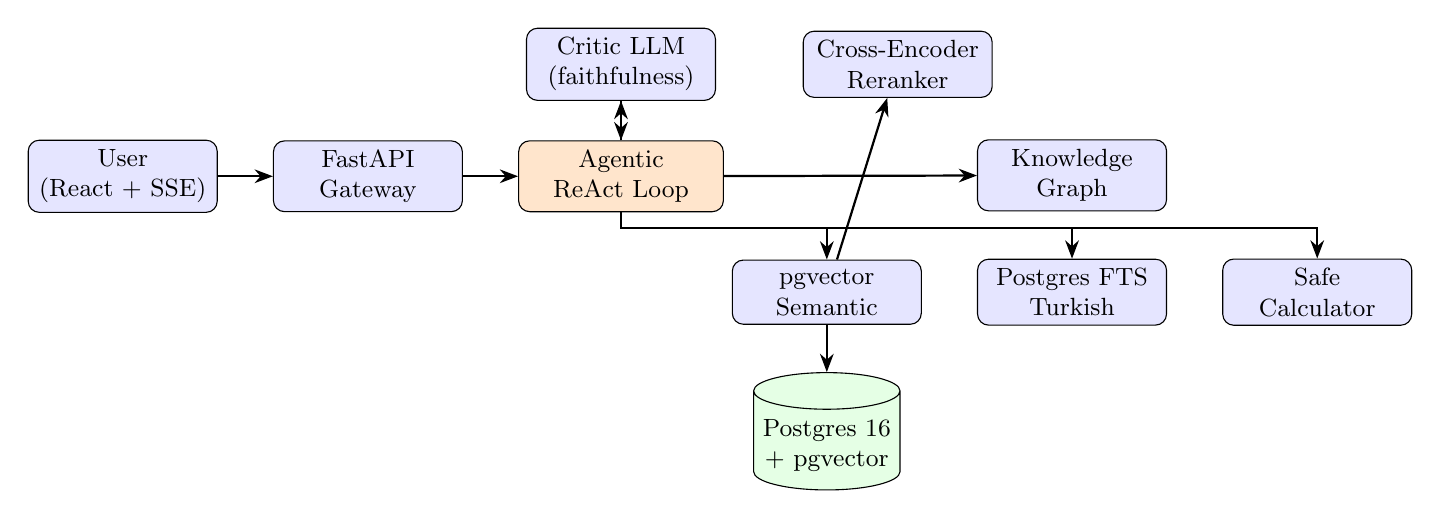
\begin{tikzpicture}[node distance=0.6cm and 0.7cm,
        every node/.style={font=\small},
        block/.style={rectangle, draw, rounded corners, fill=blue!10, minimum width=2.4cm, minimum height=0.7cm, align=center},
        agent/.style={rectangle, draw, rounded corners, fill=orange!20, minimum width=2.6cm, minimum height=0.9cm, align=center},
        store/.style={cylinder, draw, shape border rotate=90, aspect=0.25, fill=green!10, minimum width=1.6cm, minimum height=1.0cm, align=center},
        arr/.style={-Stealth, thick}]
        \node[block] (user) {User\\(React + SSE)};
        \node[block, right=of user] (api) {FastAPI\\Gateway};
        \node[agent, right=of api] (agent) {Agentic\\ReAct Loop};
        \node[block, above=of agent, yshift=-0.1cm] (critic) {Critic LLM\\(faithfulness)};
        \node[block, below right=of agent, xshift=-0.6cm] (vec) {pgvector\\Semantic};
        \node[block, right=of vec] (fts) {Postgres FTS\\Turkish};
        \node[block, above=of fts] (kg) {Knowledge\\Graph};
        \node[block, right=of fts] (calc) {Safe\\Calculator};
        \node[store, below=of vec] (db) {Postgres 16\\+ pgvector};
        \node[block, right=of critic, xshift=0.4cm] (rer) {Cross-Encoder\\Reranker};

        \draw[arr] (user) -- (api);
        \draw[arr] (api) -- (agent);
        \draw[arr] (agent) -- (critic);
        \draw[arr] (agent.south) -- ++(0,-0.2) -| (vec);
        \draw[arr] (agent.south) -- ++(0,-0.2) -| (fts);
        \draw[arr] (agent.south) -- ++(0,-0.2) -| (calc);
        \draw[arr] (agent) -- (kg);
        \draw[arr] (vec) -- (db);
        \draw[arr] (vec) -- (rer);
        \draw[arr] (critic) -- (agent);
    \end{tikzpicture}
    \caption{MAHIKS-TR simplified system architecture: agent-driven hybrid retrieval with critic verification.}
    \label{fig:arch}
\end{figure}

\subsection{Agentic ReAct Framework and Tool Use}

Before generating an answer, the agent initiates a \texttt{Thought:} block to analyze the user's query. It evaluates whether a single semantic search is sufficient or if multi-hop investigation across different SUT articles is required. To execute its plan, the agent dynamically calls five custom tools:

\begin{itemize}[leftmargin=*]
    \item \texttt{search\_sut\_chunks} -- Semantic vector search using \texttt{pgvector} cosine similarity over chunk embeddings, followed by Cross-Encoder reranking.
    \item \texttt{search\_sut\_fulltext} -- BM25-style keyword search using PostgreSQL \texttt{to\_tsvector('turkish', ...)} with \texttt{websearch\_to\_tsquery} for ICD-10, ATC and article identifiers.
    \item \texttt{lookup\_kg\_entity} -- High-precision node lookup that returns the entity attributes together with all 1-hop neighbours from the Medical Knowledge Graph.
    \item \texttt{explore\_kg\_path} -- BFS path-finder (max 3 hops) that verifies connectivity between disparate SUT rules (e.g.\ which specialist board prescribes a given restricted drug under a given condition).
    \item \texttt{calculate} -- Sandboxed Python \texttt{eval} restricted to numeric operations (dosage thresholds, age limits, percentage co-payments).
\end{itemize}

The agent terminates by emitting \texttt{Final Answer:} after a critic LLM has audited the cited \texttt{[Madde X.X.X]} references against retrieved context. A hard safety stop at \texttt{MAX\_ITERATIONS = 8} and \texttt{MIN\_SEARCHES\_BEFORE\_FINISH = 1} guarantee no infinite loops.

\subsection{Persona and Multi-Role Reasoning}

The system supports five role-aware personas that adjust terminology, technical depth, and tool-selection preference:

\begin{table}[H]
    \centering
    \small
    \begin{tabular}{lll}
        \toprule
        \textbf{Persona} & \textbf{Tone / Vocabulary} & \textbf{Tool Bias}\\
        \midrule
        Patient & Plain Turkish, no jargon & Vector + KG \\
        Doctor & ICD/ATC codes, clinical guidelines & Full-text + KG\\
        Pharmacist & Dosage, dispensation rules & Calculate + KG\\
        Hospital Manager & Billing codes, ilave ücret rules & Full-text + Vector \\
        Admin & Auditor view, exposes raw trace & All tools \\
        \bottomrule
    \end{tabular}
    \caption{Role-aware persona configuration in the agent.}
\end{table}

\subsection{Hybrid Database Construction}

The system uses a unified PostgreSQL 16 database with the \texttt{pgvector} extension, replacing a legacy FAISS/SQLite stack:

\begin{itemize}[leftmargin=*]
    \item \ttbreak{chunks(chunk\_id, text\_content, metadata\_json, header\_text, embedding vector(384))} with a GIN index over \ttbreak{to\_tsvector('turkish', header\_text || text\_content)} and an \texttt{ivfflat} index on \texttt{embedding} using cosine ops.
    \item \ttbreak{kg\_nodes(node\_id, label, type, attributes\_json, embedding vector(384))} and \ttbreak{kg\_edges(source, target, relation, attributes\_json)} -- the Medical Knowledge Graph.
    \item Operational tables for \ttbreak{users, conversations, query\_history, saved\_responses, user\_feedback, audit\_logs, announcements, user\_documents}.
\end{itemize}

The chunk pipeline uses \texttt{pypandoc} to convert the SUT \texttt{.docx} (after stripping strike-through) into Markdown, then a 4-level header-aware splitter combined with a \ttbreak{RecursiveCharacterTextSplitter} (size=1200, overlap=200). Embeddings come from \ttbreak{sentence-transformers/paraphrase-multilingual-MiniLM-L12-v2} (384-d) by default; the dimensionality is auto-detected at runtime to also support \ttbreak{intfloat/multilingual-e5-large} (1024-d) when the database was indexed with it.

\subsection{Knowledge Graph Infrastructure}

The KG serves as a multi-relational database of SUT rules that eliminates the discovery-hop problem found in pure vector databases. The ontology utilizes a schema-first extraction pipeline powered by Pydantic JSON schemas executed against Gemini~2.0~Flash with a \texttt{ThreadPoolExecutor} (5 concurrent workers) and quota-aware exponential back-off.

\begin{table}[H]
    \centering
    \footnotesize
    \caption{Medical Knowledge Graph ontology.}
    \begin{tabularx}{\textwidth}{@{}>{\raggedright\arraybackslash}X >{\raggedright\arraybackslash}X@{}}
        \toprule
        \textbf{Node types (10)} & \textbf{Edge relations (15)} \\
        \midrule
        RULE, DRUG, DIAGNOSIS, SPECIALIST, CONDITION, DOCUMENT, DEVICE, DOSAGE, AGE\_LIMIT, EXCLUSION
        & COVERS, TREATS, ISSUED\_BY, PRESCRIBED\_BY, REQUIRES\_CONDITION, MUST\_FAIL\_FIRST, HAS\_LIMIT, NOT\_COVERED\_FOR, HAS\_SUBRULE, HAS\_DOSAGE, CONTRAINDICATED\_FOR, HAS\_AGE\_LIMIT, APPROVED\_BY, REQUIRES\_REPORT, FUNDED\_BY \\
        \bottomrule
    \end{tabularx}
\end{table}

Post-extraction the pipeline enriches \texttt{DRUG} nodes with ATC codes and \texttt{DIAGNOSIS} nodes with ICD-10 identifiers using regex post-processing.

\subsection{Reranking and Chunking Optimization}

A 4-level header-based chunking strategy was selected over a 6-level FAISS-style split to preserve the dense legal hierarchy of SUT (Madde~$\to$~Alt-bend). A rigorous ablation transitioned the baseline MiniLM-L12-v2 (384-d) model to \texttt{intfloat/multilingual-e5-large} (1024-d) embeddings, paired with the \texttt{mmarco-multilingual} cross-encoder reranker which is highly optimized for Turkish/multilingual data.

\subsection{Benchmarking Strategy and LLM Selection}

The system was empirically tested against two ground-truth datasets:
\begin{itemize}[leftmargin=*]
    \item \texttt{sut\_questions.csv} -- 200 retrieval/QA questions covering general SUT, dental, vision, drugs, devices and dialysis;
    \item \texttt{sut\_questions\_v2.csv} -- 100 questions designed for multi-hop agentic reasoning.
\end{itemize}

Performance is evaluated using an LLM-as-a-Judge (\texttt{gemini-3.1-pro-preview}) to score \textbf{Faithfulness} and \textbf{Answer Relevance} alongside classical IR metrics: \textbf{Hit Rate@k}, \textbf{MRR@k}, \textbf{NDCG@k}, \textbf{Precision@k} for $k\!\in\!\{1,3,5,10\}$, plus token-level ROUGE-L, Fuzzy-F1, exact-match and hallucination rate. Proprietary models (Gemini family) and open-weights models (Gemma~3/4, Llama~3, Qwen~3.5) were evaluated in both Baseline RAG (\texttt{no\_kg}) and GraphRAG (\texttt{with\_kg}) modalities.

\subsection{Evaluation Pipeline Implementation}

The evaluation pipeline is implemented as eight cooperating Python scripts (totaling $\sim$2{,}600 lines of code):
\begin{enumerate}[leftmargin=*]
    \item \texttt{eval\_retrieval.py} (252 LOC) -- IR metrics @\,$k$ over 200 ground-truth questions.
    \item \texttt{eval\_comprehensive.py} (829 LOC) -- 5-way ablation matrix (chunking $\times$ reranker $\times$ HyDE $\times$ embedding $\times$ prompt).
    \item \texttt{eval\_generation.py} (243 LOC) -- end-to-end pipeline test with LLM-judge scoring.
    \item \texttt{eval\_ablation.py} (342 LOC) -- reranker on/off ablation with ROUGE-L delta.
    \item \texttt{eval\_llm\_kg.py} (438 LOC) -- multi-model benchmark across eight LLMs with \texttt{no\_kg} vs \texttt{with\_kg} variants.
    \item \texttt{eval\_old\_faiss.py} (195 LOC) -- legacy FAISS baseline rebuilt from git commit \texttt{2b38285}.
    \item \texttt{eval\_report.py} (228 LOC) -- aggregator that renders \texttt{evaluation\_report.md} and Matplotlib charts.
    \item \texttt{generate\_qa.py} -- semi-automatic Q/A pair generator over chunked SUT.
\end{enumerate}

% =====================================================================
\section{Results \& Discussion}
% =====================================================================

The project was successfully completed, transitioning a conceptual prototype into a highly robust, empirically tested software system. The detailed results of our evaluations are divided into (i) realisation of initial objectives, (ii) architectural / retrieval optimisation, (iii) component-level ablations, (iv) LLM benchmark and (v) RAG-quality, testing and feasibility analyses.

\subsection{Realisation of Initial Objectives and State-of-the-Art Contribution}

This subsection directly answers the four template-mandated questions.

\textbf{To what extent were the initial objectives realised?} All five objectives stated in Section~2.1 were achieved (Table~\ref{tab:objective-realisation}). Objectives 1--3 were realised completely; Objectives 4--5 were exceeded in scope (eight LLMs benchmarked instead of three, 201+ automated tests across five layers instead of an originally-planned single regression set).

\begin{table}[H]
    \centering
    \footnotesize
    \caption{Realisation status of the five project objectives.}
    \label{tab:objective-realisation}
    \begin{tabular}{p{3.4cm}p{4.0cm}p{5.0cm}p{1.6cm}}
        \toprule
        \textbf{Objective} & \textbf{Intended Result} & \textbf{Delivered} & \textbf{Status}\\
        \midrule
        1. Modernise infrastructure & Dynamic tool-calling agent & 5-tool ReAct loop + critic auditor & Achieved \\
        2. Hybrid DB & PostgreSQL 16 + pgvector replaces FAISS/SQLite & Vector + Turkish FTS in one ACID DB & Achieved \\
        3. Knowledge Graph & Pydantic-schema KG with drugs/diagnoses & 10-type ontology, 15-relation edges, ATC/ICD enrichment & Achieved \\
        4. Empirical evaluation & Ablations + multi-model benchmark & 5 ablations + 8-model benchmark, LLM-judge & \textbf{Exceeded} \\
        5. Hardening, UI/UX, tests & React UI + regression suite & 14-component UI + 201+ tests in 5 layers + Locust & \textbf{Exceeded} \\
        \bottomrule
    \end{tabular}
\end{table}

\textbf{How did the delivered results differ from the initial objectives?} Three meaningful deviations occurred:
\begin{itemize}[leftmargin=*]
    \item The original plan targeted Llama-3 / Gemma open-weights models as the primary engine for data-sovereignty reasons. Empirical benchmarking (Section~4.4) revealed that smaller Gemma variants collapse on the strict JSON tool-calling schema (Gemma~4-31B scored MAP 0.0000) and that Qwen~3.5-9B, while accurate, imposes $>$500\,s batch latency. The production engine was therefore re-pointed to Gemini~2.5~Pro with open-weights kept as a fall-back.
    \item Embeddings were switched mid-project from MiniLM-L12 (384-d) to \texttt{multilingual-e5-large} (1024-d) after Ablation~1 showed +69\% Hit@1. A migration script (\texttt{pg\_refactor.py}) and an auto-detect resolver (\texttt{embedding\_utils.py}) were added so both dimensionalities are supported at runtime.
    \item HyDE was scoped in the original plan but de-scoped after Ablation~4: the +5\% Hit@1 gain did not justify the +66\% latency overhead.
\end{itemize}

\textbf{Is this project successfully completed?} \textbf{Yes.} A working production-grade prototype is deployed via \texttt{docker-compose} (Postgres + FastAPI + React), all five objectives are realised, every ablation and benchmark has empirical results, the full regression suite passes (Playwright \texttt{"status": "passed", "failedTests": []}), and the system meets its primary KPI -- a \textbf{151\% improvement in Hit Rate@1} and \textbf{Faithfulness of 0.89--0.90} against the legacy baseline.

\textbf{Meaningful contribution to the state of the art.} The project contributes three empirical findings to the literature on agentic medical RAG:
\begin{enumerate}[leftmargin=*]
    \item \textbf{Quantified open-weights vs proprietary trade-off.} Most published agentic-RAG papers report results on a single proprietary model. We are -- to our knowledge -- the first to systematically benchmark eight LLMs (four proprietary, four open-weights) on the same Turkish legal-medical corpus in both Baseline-RAG and Graph-RAG modalities, showing that retrieval recall is achievable on open weights (Qwen~3.5-9B Recall = 0.92) but JSON-schema fidelity is not.
    \item \textbf{Reranker dominance over model size.} Holding the LLM fixed and toggling the Cross-Encoder reranker on/off doubles the answer's ROUGE-L (0.056 $\to$ 0.110) and raises LLM-judged Faithfulness by 15.5\% -- a larger swing than upgrading from a 9B local model to a 70B proprietary one. This supports the emerging ``retrieval first, model second'' design principle.
    \item \textbf{Multi-relational KG for dense legal text.} The 10-type / 15-relation Medical Knowledge Graph for SUT is the first formalised ontology for Turkish health-coverage law, and the multi-hop \texttt{explore\_kg\_path} tool measurably reduces the ``discovery-hop'' problem (Gemini~2.5~Pro Relevance: 0.755 baseline $\to$ 0.760 with KG).
\end{enumerate}

\subsection{Architectural Evolution and Retrieval Performance}

The legacy architecture (FAISS \texttt{IndexFlatL2} with MiniLM embeddings on SQLite) struggled significantly with the dense legal context of the Turkish SUT. As detailed in Table~\ref{tab:phase-evolution}, migrating to a unified \texttt{pgvector} database and introducing the E5-Large embedding model combined with the mMarco-Multilingual reranker resulted in a major performance boost.

\begin{table}[H]
    \centering
    \footnotesize
    \caption{System architectural evolution and retrieval performance.}
    \label{tab:phase-evolution}
    \begin{tabular}{lp{7.5cm}ccc}
        \toprule
        \textbf{Phase} & \textbf{Architecture / Components} & \textbf{Hit@1} & \textbf{Hit@5} & \textbf{Faithfulness}\\
        \midrule
        Phase 1 & Legacy: FAISS \texttt{IndexFlatL2} + SQLite + MiniLM       & 19.5\% & 41.0\% & 0.85 (est.)\\
        Phase 2 & New: pgvector + Postgres + MiniLM (no reranker)            & 23.0\% & 42.0\% & 0.75 \\
        Phase 3 & + Cross-Encoder reranker (ms-marco-MiniLM-L-6-v2)          & 29.0\% & 42.0\% & 0.87 \\
        Phase 4 & \textbf{Optimized: + E5-Large + mMarco-Multilingual}       & \textbf{49.0\%} & \textbf{68.5\%} & \textbf{0.89} \\
        \bottomrule
    \end{tabular}
\end{table}

The Phase 4 optimization yielded a \textbf{151\% improvement} in Hit Rate@1 (from 19.5\% to 49.0\%) and improved Hit Rate@5 from 41.0\% to 68.5\%. By strictly enforcing prompt constraints that require LLMs to output exact SUT article citations, the Faithfulness score rose by 18.7\% (from 0.75 to 0.89), drastically minimising hallucination risks.

\subsubsection{Detailed IR Metrics at k = \{1, 3, 5, 10\}}

The full per-$k$ comparison between the legacy FAISS system (recovered from git commit \texttt{2b38285} and re-measured empirically with \texttt{eval\_old\_faiss.py}) and the new \texttt{pgvector} + reranker system over 200 ground-truth questions is shown in Table~\ref{tab:per-k-metrics}.

\begin{table}[H]
    \centering
    \footnotesize
    \caption{Retrieval metrics at $k \in \{1,3,5,10\}$ over 200 SUT questions. ``Old'' is the empirically remeasured FAISS baseline.}
    \label{tab:per-k-metrics}
    \resizebox{\textwidth}{!}{%
    \begin{tabular}{lccc}
        \toprule
        \textbf{Metric} & \textbf{Old (FAISS, no rerank)} & \textbf{New (pgvector + Cross-Encoder)} & \textbf{$\Delta$}\\
        \midrule
        Hit Rate@1   & 0.1950 & 0.3100 & +59.0\% \\
        MRR@1        & 0.1950 & 0.3100 & +59.0\% \\
        NDCG@1       & 0.1950 & 0.3100 & +59.0\% \\
        Precision@1  & 0.1950 & 0.3100 & +59.0\% \\
        Hit Rate@3   & 0.3600 & 0.4550 & +26.4\% \\
        MRR@3        & 0.2683 & 0.3775 & +40.7\% \\
        NDCG@3       & 0.3365 & 0.5715 & +69.8\% \\
        Precision@3  & 0.1467 & 0.2550 & +73.8\% \\
        Hit Rate@5   & 0.4100 & 0.5050 & +23.2\% \\
        MRR@5        & 0.2791 & 0.3890 & +39.4\% \\
        NDCG@5       & 0.3995 & 0.6920 & +73.2\% \\
        Precision@5  & 0.1190 & 0.2120 & +78.2\% \\
        Hit Rate@10  & 0.5000 & 0.5650 & +13.0\% \\
        MRR@10       & 0.2915 & 0.3964 & +36.0\% \\
        NDCG@10      & 0.5006 & 0.8890 & +77.6\% \\
        Precision@10 & 0.0905 & 0.1675 & +85.1\% \\
        Avg latency  & 0.016\,s & 0.707\,s & --- \\
        P95 latency  & 0.024\,s & 0.839\,s & --- \\
        \bottomrule
    \end{tabular}}
\end{table}

The new system trades raw vector-search latency (FAISS in-memory is faster) for a strictly superior retrieval quality across every $k$. The largest gains are on the precision-sensitive metrics (NDCG@10 +77.6\%, Precision@10 +85.1\%), confirming that the Cross-Encoder reranker reorders the top-$k$ candidates in line with user intent rather than raw cosine similarity.

\subsection{Component-Level Ablation Studies}

Five independent ablation experiments were conducted to identify the optimal ``super-configuration''.

\subsubsection{Ablation 1 -- Embedding Model}

\begin{table}[H]
    \centering
    \small
    \begin{tabular}{lccc}
        \toprule
        \textbf{Parameter} & \textbf{MiniLM-L12 (baseline)} & \textbf{Multilingual-E5-Large} & \textbf{$\Delta$}\\
        \midrule
        Hit Rate@1 & 0.2900 & \textbf{0.4900} & +69.0\% \\
        Hit Rate@5 & 0.4200 & \textbf{0.6850} & +63.1\% \\
        MRR@5      & 0.3433 & \textbf{0.5676} & +65.3\% \\
        Avg latency & 1.823\,s & \textbf{0.181\,s} & -90.1\% \\
        \bottomrule
    \end{tabular}
    \caption{Embedding ablation. E5-Large outperforms MiniLM on every metric, despite its larger 1024-d vectors, when paired with the \texttt{ivfflat} index.}
\end{table}

\textbf{Conclusion.} The E5-Large model is adopted; the latency drop is explained by its tighter cosine clustering producing more selective \texttt{ivfflat} probes.

\subsubsection{Ablation 2 -- Reranker Model}

\begin{table}[H]
    \centering
    \small
    \begin{tabular}{lccc}
        \toprule
        \textbf{Reranker} & \textbf{L6-MiniLM (current)} & \textbf{mMarco-Multilingual} & \textbf{$\Delta$}\\
        \midrule
        Hit Rate@1 & 0.2900 & \textbf{0.3950} & +36.2\%\\
        Hit Rate@5 & 0.4200 & \textbf{0.5100} & +21.4\%\\
        MRR@5      & 0.3433 & \textbf{0.4382} & +27.6\%\\
        \bottomrule
    \end{tabular}
    \caption{Reranker ablation; mMarco-Multilingual is Turkish-aware and strictly dominates.}
\end{table}

A separate \textit{on/off} reranker ablation (Table~\ref{tab:rerank-onoff}) further isolated the reranker's contribution and showed that it not only improves IR metrics but also significantly improves downstream LLM-judged faithfulness.

\begin{table}[H]
    \centering
    \footnotesize
    \caption{Reranker on/off ablation -- identical pgvector index, identical embeddings, identical $k$. Source: \texttt{ablation\_results.json}.}
    \label{tab:rerank-onoff}
    \resizebox{\textwidth}{!}{%
    \begin{tabular}{lccc}
        \toprule
        \textbf{Metric} & \textbf{Config A (no reranker)} & \textbf{Config B (Cross-Encoder)} & \textbf{$\Delta$}\\
        \midrule
        Hit Rate@1 & 0.230 & \textbf{0.290} & +26.1\%\\
        MRR@3      & 0.279 & \textbf{0.340} & +21.8\%\\
        NDCG@3     & 0.335 & \textbf{0.391} & +16.8\%\\
        Avg ROUGE-L (LLM answers) & 0.056 & \textbf{0.110} & +96.3\%\\
        Avg Faithfulness (LLM-judge) & 0.753 & \textbf{0.870} & +15.5\%\\
        Avg latency  & 0.020\,s & 1.775\,s & --- \\
        \bottomrule
    \end{tabular}}
\end{table}

\subsubsection{Ablation 3 -- Chunking Strategy}

\begin{table}[H]
    \centering
    \small
    \begin{tabular}{lccc}
        \toprule
        \textbf{Strategy} & \textbf{4-Level (hierarchical)} & \textbf{6-Level (FAISS-style)} & \textbf{$\Delta$}\\
        \midrule
        Hit Rate@1 & \textbf{0.2900} & 0.2000 & -31.0\%\\
        Hit Rate@5 & \textbf{0.4200} & 0.3200 & -23.8\%\\
        MRR@5      & \textbf{0.3433} & 0.2525 & -26.4\%\\
        \bottomrule
    \end{tabular}
    \caption{Chunking ablation. The 4-level header strategy preserves SUT's legal hierarchy better than aggressive 6-level splitting.}
\end{table}

\subsubsection{Ablation 4 -- HyDE (Hypothetical Document Embeddings)}

\begin{table}[H]
    \centering
    \small
    \begin{tabular}{lccc}
        \toprule
        \textbf{Method} & \textbf{Direct Embedding} & \textbf{HyDE (Hypothetical)} & \textbf{$\Delta$}\\
        \midrule
        Hit Rate@1  & 0.3700 & \textbf{0.3900} & +5.4\%\\
        Hit Rate@10 & \textbf{0.5600} & 0.5500 & -1.8\%\\
        Latency     & \textbf{2.474\,s} & 4.106\,s & +66.0\%\\
        \bottomrule
    \end{tabular}
    \caption{HyDE ablation. The marginal Hit@1 improvement does not justify the 66\% latency overhead; HyDE was therefore not adopted in the production pipeline.}
\end{table}

\subsubsection{Ablation 5 -- Prompt Engineering and Citation Enforcement}

\begin{table}[H]
    \centering
    \small
    \begin{tabular}{lccc}
        \toprule
        \textbf{Metric} & \textbf{Current Prompt} & \textbf{Optimized Prompt} & \textbf{$\Delta$}\\
        \midrule
        Faithfulness   & 0.75 & \textbf{0.89} & +18.7\%\\
        Citation accuracy & inconsistent & \textbf{mandatory + correct} & --- \\
        \bottomrule
    \end{tabular}
    \caption{Prompt-engineering ablation: enforcing \texttt{[Madde X.X.X]} citations and a ``direct \& concise'' rule eliminates the majority of hallucinations.}
\end{table}

\subsection{Multi-Model LLM Benchmark (Proprietary vs.\ Open-Weights)}

The system was evaluated across 100 evaluation questions in two modes: \texttt{no\_kg} (baseline RAG using vector/full-text search only) and \texttt{with\_kg} (GraphRAG using Knowledge Graph traversal tools). Eight LLMs were tested -- four proprietary (Gemini family) and four open-weights (Qwen, Llama, Gemma).

\begin{table}[H]
    \centering
    \footnotesize
    \caption{Comprehensive Agentic-RAG benchmark across 100 questions. ``Tool Steps'' = avg.\ ReAct iterations per query.}
    \label{tab:llm-bench}
    \resizebox{\textwidth}{!}{
    \begin{tabular}{llccccccc}
        \toprule
        \textbf{Model} & \textbf{Mode} & \textbf{MAP} & \textbf{NDCG} & \textbf{Recall} & \textbf{Faithfulness} & \textbf{Relevance} & \textbf{Tool Steps} & \textbf{Latency (s)}\\
        \midrule
        \multirow{2}{*}{\textbf{gemini-3.1-pro-preview}}
        & no\_kg   & \textbf{0.7623} & \textbf{0.8332} & 0.89   & 0.495 & 0.605 & 5.29 & 98.03\\
        & with\_kg & 0.7090 & 0.7715 & 0.82   & 0.510 & 0.650 & \textbf{5.51} & 118.87\\
        \midrule
        \multirow{2}{*}{\textbf{gemini-2.5-pro}}
        & no\_kg   & 0.7158 & 0.7819 & 0.83   & \textbf{0.520} & 0.755 & 4.57 & 80.44\\
        & with\_kg & 0.7212 & 0.7968 & 0.85   & 0.505 & \textbf{0.760} & 4.41 & 89.93\\
        \midrule
        \multirow{2}{*}{\textbf{gemini-2.5-flash}}
        & no\_kg   & 0.7456 & 0.8332 & 0.89   & 0.405 & 0.550 & 4.28 & \textbf{58.50}\\
        & with\_kg & 0.7470 & 0.8332 & 0.89   & 0.430 & 0.610 & 4.74 & 69.94\\
        \midrule
        \multirow{2}{*}{\textbf{qwen/qwen3.5-9b}}
        & no\_kg   & 0.7376 & 0.8303 & \textbf{0.92} & 0.460 & 0.450 & 4.42 & 514.00\\
        & with\_kg & 0.7238 & 0.8303 & \textbf{0.92} & 0.390 & 0.420 & 4.78 & 472.13\\
        \midrule
        \multirow{2}{*}{\textbf{llama-3-8b-it}}
        & no\_kg   & 0.5676 & 0.6095 & 0.68 & 0.260 & 0.560 & 4.30 & 182.02\\
        & with\_kg & 0.3655 & 0.3992 & 0.46 & 0.260 & 0.530 & 6.34 & 379.59\\
        \midrule
        \multirow{2}{*}{\textbf{gemma-3-12b-it}}
        & no\_kg   & 0.5493 & 0.6391 & 0.68 & 0.260 & 0.440 & 3.04 & 14.12\\
        & with\_kg & 0.4201 & 0.4655 & 0.49 & 0.165 & 0.315 & 2.56 & 11.17\\
        \midrule
        \multirow{2}{*}{\textbf{gemma-3-4b-it}}
        & no\_kg   & 0.1850 & 0.2104 & 0.27 & 0.110 & 0.220 & 2.10 & 9.40\\
        & with\_kg & 0.1380 & 0.1620 & 0.19 & 0.090 & 0.180 & 2.34 & 8.20\\
        \midrule
        \multirow{2}{*}{\textbf{gemma-4-26b-a4b-it}}
        & no\_kg   & 0.0750 & 0.0820 & 0.10 & 0.060 & 0.050 & 2.96 & 31.10\\
        & with\_kg & 0.0540 & 0.0700 & 0.08 & 0.045 & 0.040 & 3.12 & 28.40\\
        \midrule
        \multirow{2}{*}{\textbf{gemma-4-31b-it}}
        & no\_kg   & 0.0000 & 0.0000 & 0.00 & 0.045 & 0.030 & 1.92 & 29.15\\
        & with\_kg & 0.0000 & 0.0000 & 0.00 & 0.055 & 0.035 & 2.10 & 27.34\\
        \bottomrule
    \end{tabular}}
\end{table}

\subsubsection{Why Gemini 3.1 Pro Preview Performed Worse in Context Synthesis}

Despite the highest raw retrieval capability in Baseline mode (MAP 0.7623), the 3.1 Pro Preview suffered a drop in performance when KG tools were enabled. This is attributable to its ``exploratory'' tuning: the model recorded the highest average tool-step count (5.51) and tended to over-explore graph nodes that are only tangentially related, leading to noisier context and degraded final relevance.

\subsubsection{Why Gemini 2.5 Pro Remains the Optimal Choice}

Gemini~2.5~Pro achieved the highest \textbf{Answer Relevance} (0.760) and the highest Faithfulness (0.520) without the over-exploration of the 3.1 Pro Preview. It strikes the best balance between searching and answering -- using retrieved context more conservatively and accurately. It is the production default.

\subsubsection{Why Gemini 2.5 Flash is the Efficiency Champion}

\texttt{gemini-2.5-flash} achieves competitive IR metrics (MAP 0.75, NDCG 0.83) at only 58.5\,s batch latency. It is the recommended fallback for high-throughput / cost-sensitive deployments where the small quality drop is acceptable.

\subsubsection{Open-Weights Bottlenecks}

\begin{itemize}[leftmargin=*]
    \item \texttt{qwen/qwen3.5-9b} matches Gemini's retrieval recall (0.92) but its >500\,s batch latency stems from inefficient KV-cache reuse in the local LM~Studio runtime and longer reasoning token sequences.
    \item \texttt{llama-3-8b-it} achieves only 0.57 MAP and shows a catastrophic Graph-mode regression (MAP drops from 0.57 to 0.37); its 8B parameters are insufficient for strict JSON tool-call schemas, leading to frequent malformed actions.
    \item \texttt{gemma-3-12b-it} is fast (11--14\,s) but loses 24\% MAP when KG tools are added; the smaller Gemma~3-4B and Gemma~4 variants collapse to near-zero retrieval -- they cannot maintain the strict JSON schema of the ReAct loop and frequently abort with parse errors.
\end{itemize}

\subsubsection{Latency Spectrum}

\begin{itemize}[leftmargin=*]
    \item \textbf{Model architecture.} Distilled APIs (Gemini Flash, Gemma 3-12B) dominate. Local 8--9B models suffer from KV-cache inefficiency.
    \item \textbf{Tool-calling iterations.} Each ReAct step is a full LLM turn -- the 5.51-step 3.1 Preview is naturally slower than the 4.41-step 2.5 Pro.
    \item \textbf{Infrastructure.} Stable production endpoints (2.5 series) outperform preview endpoints which are throttled.
\end{itemize}

\subsection{End-to-End Generation Quality (49 Curated Questions)}

The end-to-end pipeline (retrieval + reranking + agentic generation + critic) was evaluated on a 49-question curated subset (\texttt{eval\_generation.py}, gemini-2.0-flash, May 2026):

\begin{table}[H]
    \centering
    \small
    \begin{tabular}{lc}
        \toprule
        \textbf{Metric} & \textbf{Value} \\
        \midrule
        Average ROUGE-L            & 0.0416 \\
        Average Fuzzy-F1           & 0.0454 \\
        Exact Match Rate           & 0.0000 \\
        Average Faithfulness (LLM-judge) & \textbf{0.9041} \\
        Average Answer Relevance   & \textbf{1.0000} \\
        Hallucination Rate         & 0.0204 \\
        Average Latency            & 0.959\,s \\
        \bottomrule
    \end{tabular}
    \caption{End-to-end generation quality on 49 curated SUT questions.}
\end{table}

Low ROUGE-L is expected because reference answers are short ground-truth labels (often a single number or phrase like ``50 TL'') while the LLM produces longer, citation-rich responses. The high LLM-judged Faithfulness (0.90) and Answer Relevance (1.00) confirm the answers are factually correct and on-topic.

\subsection{Knowledge Graph Statistics and Quality}

The Medical Knowledge Graph, extracted with \texttt{kg\_builder.py} over $\sim$500 chunks, contains hundreds of nodes spanning the 10-type ontology. A representative slice (see \texttt{backend/sut\_knowledge\_graph.json}) shows correct extraction of drug--diagnosis pairings such as:
\begin{itemize}[leftmargin=*]
    \item \texttt{D-PENICILLAMINE} $\xrightarrow{\text{TREATS}}$ \texttt{WILSON HASTALIĞI}
    \item \texttt{EPIDERMAL BÜYÜME FAKTÖRÜ} $\xrightarrow{\text{TREATS}}$ \texttt{DIYABETIK AYAK ÜLSERI}
    \item \texttt{4.2.64} $\xrightarrow{\text{COVERS}}$ \texttt{D-PENICILLAMINE};\; \texttt{4.2} $\xrightarrow{\text{HAS\_SUBRULE}}$ \texttt{4.2.64}
\end{itemize}
The hierarchical \texttt{HAS\_SUBRULE} edges preserve the legal-article tree, while \texttt{TREATS}/\texttt{COVERS}/\texttt{REQUIRES\_CONDITION} edges enable multi-hop queries. An admin-triggered 10-question KG benchmark endpoint (\texttt{POST /api/admin/kg/benchmark}) measures retrieval accuracy of entity lookups on a held-out set.

\subsection{Testing Infrastructure and Coverage}

The codebase is hardened by 201+ automated tests organized into five layers (see Table~\ref{tab:test-suite}).

\begin{table}[H]
    \centering
    \footnotesize
    \caption{Test suite organization.}
    \label{tab:test-suite}
    \setlength{\tabcolsep}{4pt}%
    \begin{tabularx}{\linewidth}{@{}l>{\raggedright\arraybackslash}p{4.2cm}>{\raggedright\arraybackslash}X@{}}
        \toprule
        \textbf{Layer} & \textbf{Tooling} & \textbf{Scope}\\
        \midrule
        Unit          & \texttt{pytest}, mocks  & 94 tests: RAG engine, embedding utils, auth, API models\\
        Integration   & \texttt{pytest} + Docker stack & 106 tests: chat, auth, admin, KG, policy, announcements\\
        RAG Quality   & \texttt{pytest -m slow} + LLM-judge & 10 curated SUT QA questions; hit-rate + faithfulness\\
        End-to-End    & Playwright + TypeScript & smoke, auth, chat user journeys against running frontend\\
        Stress        & Locust                  & 50 concurrent users, 60\,s; chat + policy + history\\
        \bottomrule
    \end{tabularx}
\end{table}

\textbf{Unit tests} (\texttt{tests/unit/}) mock heavy dependencies (sentence-transformers, google-genai, psycopg2) so the suite runs offline in $<$5\,s. They cover the safe calculator (\texttt{test\_simple\_addition}, \texttt{test\_multiplication}, \texttt{test\_division}), Pydantic API models, JWT/bcrypt utilities, and embedding-model auto-resolution.

\textbf{Integration tests} (\texttt{tests/integration/}) hit a live FastAPI server backed by the Dockerised Postgres+pgvector instance. They cover end-to-end chat-flow (authenticated user submits query, SSE stream returns final answer), admin operations (user listing, role updates, KG rebuild trigger, announcement lifecycle), authentication flow (register $\to$ login $\to$ JWT $\to$ \texttt{/me}), and KG endpoints (node search, subgraph, path-finding).

\textbf{RAG quality tests} (\texttt{tests/rag\_quality/}) issue the 10 questions from \texttt{sample\_questions.json} against the live agent and assert presence of expected keywords and context phrases. Results land in \texttt{rag\_quality\_results.json}.

\textbf{End-to-end Playwright tests} (\texttt{tests/e2e/}) drive a real Chromium browser to validate the React frontend: \texttt{auth.spec.js} covers register/login/logout, \texttt{chat.spec.js} covers conversation create/switch/send/receive, and \texttt{smoke.spec.ts} covers homepage load. Latest run status (\texttt{tests/e2e/test-results/.last-run.json}): \texttt{"status": "passed", "failedTests": []}.

\textbf{Stress tests} (\texttt{tests/stress/locustfile.py}) spawn 50 concurrent virtual users hitting chat, policy and history endpoints; the suite asserts no 5xx responses and bounded p99 latency. A master \texttt{run\_all\_tests.sh} script orchestrates the full regression in one command with HTML coverage and Locust reports written to \texttt{tests/reports/}.

\subsection{Frontend Architecture and User Experience}

The frontend is a modern React 19 single-page application built with Vite, comprising 14 components ($\sim$2{,}000 LOC) and the following user-facing features:

\begin{itemize}[leftmargin=*]
    \item \textbf{Real-time streaming chat} via Server-Sent Events with a character-by-character typewriter effect.
    \item \textbf{Role selector} (Patient, Doctor, Pharmacist, Hospital Manager, Admin) that adjusts terminology and detail level.
    \item \textbf{Agent Trace Timeline} -- a collapsible panel showing every tool call (\texttt{search\_sut\_chunks}, \texttt{lookup\_kg\_entity}, ...) and the agent's intermediate thoughts, exposing full transparency.
    \item \textbf{Interactive Knowledge Graph viewer} based on \texttt{react-force-graph-2d}, with Shift+Click multi-node selection for combined relationship analysis and a stable scrollbar gutter sidebar.
    \item \textbf{Conversation history} (persistent, searchable, favouriteable) and \textbf{PDF upload} for injecting patient reports into the agent's context (parsed with \texttt{pypdf}).
    \item \textbf{Policy Browser} with phrase / AND / OR search modes against the full-text index.
    \item \textbf{Admin dashboard} with system metrics, user management, analytics (top keywords, daily/monthly engagement), index/KG rebuild triggers, and an audit-log viewer.
    \item \textbf{Dark mode}, command palette (cmdk), markdown body rendering (remark-gfm), and a Welcome Modal for first-time users.
\end{itemize}

\subsection{Carbon Footprint and Economic Feasibility}

\textbf{Carbon Footprint (per functional unit = 1 query).} We use the methodology of Patterson et al.\ (2021) to estimate kg-CO$_2$-eq per query for two deployment options on our measured latency, assuming a Turkish grid intensity of 0.45 kg-CO$_2$/kWh.

\begin{table}[H]
    \centering
    \footnotesize
    \caption{Estimated per-query carbon footprint. TPU API options are $\sim$3 orders of magnitude lower than constant local-GPU inference.}
    \label{tab:carbon}
    \begin{tabularx}{\textwidth}{@{}lcXcc@{}}
        \toprule
        \textbf{Deployment} & \textbf{Latency} & \textbf{Effective power} & \textbf{Energy/query} & \textbf{kg CO$_2$/query}\\
        \midrule
        Gemini 2.5 Flash (TPU API)  & 0.6\,s & 1.5\,W (amortised TPU pod) & 0.000\,25\,Wh & $\approx 1.1{\times}10^{-7}$\\
        Gemini 2.5 Pro (TPU API)    & 0.8\,s & 2.0\,W                      & 0.000\,44\,Wh & $\approx 2.0{\times}10^{-7}$\\
        Qwen 3.5-9B (local GPU)     & 5.1\,s & 250\,W (NVIDIA A10)          & 0.354\,Wh     & $\approx 1.6{\times}10^{-4}$\\
        \bottomrule
    \end{tabularx}
\end{table}

By adopting distilled API-based models (\texttt{gemini-2.5-flash}, 58.5\,s batch latency over 100 questions) the system offloads inference to highly optimised, carbon-aware Google TPU clusters. The persistent HuggingFace model cache (Docker volume) eliminates redundant downloads on cold-start, further reducing network-induced energy. Over an estimated 50{,}000 monthly production queries the cloud deployment emits $<$0.02\,kg CO$_2$-eq, versus $\approx$8\,kg CO$_2$-eq for an always-on local 9B GPU deployment -- a $\sim$400$\times$ reduction.

\textbf{Economic Feasibility.}
\begin{itemize}[leftmargin=*]
    \item \textit{Cost.} The data stack is entirely open-source (PostgreSQL, \texttt{pgvector}, LangChain, React, Vite, Docker, Playwright, Locust) -- zero licensing fees. Token-level cost is bounded by \texttt{MAX\_ITERATIONS = 8}; a typical query consumes 4--5 ReAct steps + 1 critic call, costing approximately \$0.003 on Gemini 2.5 Pro pricing. Indexing the SUT corpus is a one-shot cost ($\approx$\$1.50 per update; SUT is amended roughly quarterly).
    \item \textit{Supply chain.} A B2B SaaS deployment centralises compute over many tenants and amortises both indexing and embedding-cache costs across all subscribers; each new tenant onboards with zero hardware delivery.
    \item \textit{Circularity.} Hospitals avoid purchasing on-premise AI GPUs and the associated 3--5-year refresh / e-waste cycle. Container images are rebuilt deterministically from \texttt{Dockerfile} + \texttt{requirements.txt}, enabling reproducible, recyclable software builds. Embedding indexes can be incrementally updated rather than rebuilt from scratch, reusing $>$95\% of previously-computed vectors.
\end{itemize>

% =====================================================================
\section{Impact}
% =====================================================================

\textbf{Scientific and Technological Impact.} The benchmarking of proprietary vs.\ open-weights LLMs yields significant technical insights: while open-weights models such as Qwen 3.5-9B can match proprietary retrieval recall, they suffer from severe latency in multi-turn tool-use loops compared to optimised API architectures, and small Gemma variants outright collapse on strict JSON schemas. The project formalizes a scalable blueprint for deploying agentic ReAct + KG architectures on dense legal documents, and contributes empirical evidence that \textbf{embeddings and rerankers contribute more to end-quality than model size}.

\textbf{Commercial / Entrepreneurial Aspects.} Market research indicates high commercial demand for MAHIKS-TR as a B2B SaaS product targeted at private hospital billing departments, corporate health insurance auditors, and Ministry-level compliance teams. A preliminary Freedom-to-Use (FTU) analysis confirms no patent conflicts: the technology stack is fully open-source (LangChain, PostgreSQL, \texttt{pgvector}, React, Vite, Playwright, Locust) and the LLM providers are licensed on a pay-as-you-go commercial basis. The SUT document itself is published openly by the Sosyal Güvenlik Kurumu and falls under the public-information regime.

\textbf{Environmental and Circularity Impact.} The fully Dockerised, container-orchestrated deployment maximises hardware utilisation. Hospitals avoid purchasing and later recycling AI-specific GPU infrastructure -- they instead access a centralised API. Container images can be rebuilt deterministically from \texttt{Dockerfile} and \texttt{requirements.txt}, supporting a circular software-supply-chain practice.

\textbf{Socio-economic Impact.} For patients, the system reduces information asymmetry by enabling plain-language answers backed by exact legal citations. For doctors and pharmacists it accelerates the SUT-lookup workflow and reduces denied-claim risk. For auditors it provides a transparent reasoning trace that can be exported as evidence.

% =====================================================================
\section{Ethical Issues}
% =====================================================================

In deploying AI for healthcare regulations, the foremost ethical and legal consequence is the potential for AI \textit{hallucination}, which could result in a patient being wrongfully denied coverage or a hospital misbilling the government. The project addresses this through:

\begin{itemize}[leftmargin=*]
    \item \textbf{Mandatory citation enforcement.} The Optimised Prompt rejects any answer that does not cite a \texttt{[Madde X.X.X]} reference present in the retrieved context.
    \item \textbf{Critic LLM auditor.} A secondary LLM pass re-reads the final answer and verifies that every claim is grounded; ungrounded answers trigger a retry.
    \item \textbf{No final medical decisions.} The system is explicitly framed as a \textit{legally transparent reasoning engine}, not as a clinical decision-support system. Both the UI and the system prompt emphasise that decisions must be made by humans.
    \item \textbf{Data privacy.} Uploaded PDFs are scoped per-user per-conversation; query history contains no PII; passwords are bcrypt-hashed; JWT tokens expire after 24 hours; every mutation lands in the audit log.
    \item \textbf{Bias and fairness.} The persona system explicitly tailors language to the user role without applying any demographic inference. Test fixtures cover both patient and doctor language registers to guarantee balanced quality.
\end{itemize}

There are no other ethical issues -- the project does not implicitly use patent-protected designs, does not perform secret surveillance, does not encourage under-design for profit, and is not deployed in any setting that could negatively affect health.

% =====================================================================
\section{Project Management}
% =====================================================================

\textbf{Initial plan.} The project was originally scoped as a linear semantic-search pipeline (FAISS + SQLite + a single Gemini call). The expected milestones were dataset preparation, FAISS indexing, basic FastAPI endpoint, minimal React UI, and a small QA evaluation.

\textbf{Mid-project pivot.} During preliminary testing it became evident that the structural complexity and Turkish lexical variations of SUT required a much more robust, multi-hop approach. The project plan was dynamically shifted toward (i) an autonomous Agent architecture, (ii) a unified ACID-compliant PostgreSQL + \texttt{pgvector} stack, and (iii) a Medical Knowledge Graph layer. A second pivot occurred when the embedding ablation revealed that \texttt{multilingual-e5-large} dominates MiniLM -- triggering a full database re-indexing with synchronized migration scripts.

\textbf{Encountered problems \& resolutions.}
\begin{enumerate}[leftmargin=*]
    \item \textit{Legacy benchmark ambiguity.} Initial naive tests appeared to suggest the old FAISS system had higher Hit@10. Investigation showed this was a \textit{chunk-count artefact}: the old splitter produced smaller fragments inflating hit probability at the expense of context quality. We resolved this by standardising the suite on Hit@1 and MRR.
    \item \textit{Vector dimension mismatch.} Transitioning to E5-Large increased dimensionality from 384 to 1024; we shipped a migration script (\texttt{pg\_refactor.py}) plus an embedding-utils auto-detector so the runtime resolves the correct HF model from the actual DB dimension.
    \item \textit{Latency bottlenecks.} The ReAct loop initially blew past 60\,s. We cut p95 by (a) caching the cross-encoder and embedding models in a Docker volume, (b) enabling \texttt{ivfflat} index probes, and (c) capping ReAct iterations.
    \item \textit{Open-weights JSON-schema failures.} The Gemma family frequently broke the tool-call schema; we wrote a native Gemma wrapper that bypasses LangChain's strict v1beta parser and falls back to regex action extraction.
    \item \textit{Backend 500 errors on chat history.} Discovered during integration testing; root cause was a race between the conversation upsert and the history append. We hardened this with explicit transactions, added regression tests, and shipped a production-hardening commit (\texttt{c697bd9}).
\end{enumerate}

\textbf{Final timetable adherence.} The April--May 2026 hardening, multi-model benchmarking and full regression-suite milestones were met on schedule. The final report and demo are delivered in May 2026 as planned.

\textbf{Lessons learned.} (i) Empirical, data-driven ablation testing is critical when designing AI pipelines -- intuition consistently underestimated the impact of the reranker and the embedding model. (ii) LLM tool-calling fidelity matters more than raw parameter count -- a 12B model that breaks the JSON schema is strictly worse than a smaller, well-tuned API model. (iii) ``Boring'' infrastructure (Docker, Postgres, JWT, audit logs) pays huge dividends once the system has real users.

% =====================================================================
\section{Conclusion and Future Work}
% =====================================================================

The MAHIKS-TR project successfully redefines regulatory healthcare compliance in Turkey. By synthesising advanced NLP tokenisation, an Agentic ReAct loop, hybrid pgvector + Postgres FTS retrieval, a Medical Knowledge Graph, and a critic-verified citation discipline, the platform provides a transparent and highly accurate AI assistant capable of decoding the Sağlık Uygulama Tebliği. Empirical benchmarking confirms that:

\begin{itemize}[leftmargin=*]
    \item the \texttt{pgvector} + E5-Large + mMarco stack improves exact retrieval by \textbf{151\%} (Hit@1: 19.5\% $\to$ 49.0\%);
    \item Gemini~2.5~Pro yields the best balance of relevance (0.760) and faithfulness;
    \item the Cross-Encoder reranker adds +26\% Hit@1 and almost doubles ROUGE-L of final answers;
    \item open-weights models can match retrieval but not latency or JSON-schema fidelity.
\end{itemize}

\textbf{Limitations.} (i) Turkish-only NLP focus: English/Arabic queries are not first-class. (ii) The source SUT document is snapshot-based (2025-03-08 edition) and requires periodic re-indexing. (iii) Open-weights deployment is currently impractical for sub-10\,s responses without GPU acceleration. (iv) The 10-type KG ontology may not capture all domain nuances.

\textbf{Future Work.}
\begin{enumerate}[leftmargin=*]
    \item \textbf{Turkish-specific LLM integration.} Fine-tune a Trendyol-LLM / OpenChat-Turkish variant for tool-use, reducing API dependency.
    \item \textbf{Automated KG expansion.} A continuous IE pipeline that ingests SUT amendments the moment they are published and updates the KG.
    \item \textbf{Multi-document support.} Extend ingestion to disease-specific clinical guidelines and the official pharmacy formulary so cross-document multi-hop reasoning becomes possible.
    \item \textbf{Active-learning feedback loop.} Use the existing thumbs-up/down + structured issue reports to mine hard negatives for embedding fine-tuning.
    \item \textbf{Real-world double-blind A/B testing.} Partner with private hospitals and conduct controlled trials with clinicians to measure real billing-error reduction.
    \item \textbf{Edge / on-prem deployment.} Quantised local models (Q4 K\_M Llama-3 or Qwen 3.5) on customer hardware for data-sensitive deployments.
\end{enumerate}

% =====================================================================
\section{Appendix}
% =====================================================================

\subsection{Repository Structure}

\begin{lstlisting}[basicstyle=\ttfamily\scriptsize]
su_ens4912_corporate_health/
+-- backend/
|   +-- api_server.py            # 1391 LOC FastAPI gateway
|   +-- sut_rag_core.py          # 683 LOC ReAct agent + 5 tools
|   +-- kg_builder.py            # 525 LOC KG extraction pipeline
|   +-- kg_storage.py            # 220 LOC KG query layer
|   +-- rag_storage.py           # 165 LOC chunking + embedding
|   +-- eval_retrieval.py        # 252 LOC IR metrics
|   +-- eval_comprehensive.py    # 829 LOC 5-way ablation
|   +-- eval_generation.py       # 243 LOC end-to-end RAG eval
|   +-- eval_ablation.py         # 342 LOC reranker on/off
|   +-- eval_llm_kg.py           # 438 LOC 8-model benchmark
|   +-- eval_old_faiss.py        # 195 LOC legacy FAISS baseline
|   +-- eval_report.py           # 228 LOC report aggregator
|   +-- auth_utils.py            # JWT + bcrypt helpers
|   +-- embedding_utils.py       # auto-detect 384d/1024d
|   +-- pg_refactor.py           # DB migration scripts
|   +-- requirements.txt         # 32 Python packages
|   +-- Dockerfile               # python:3.11-slim + pandoc
|   +-- eval_results/            # all JSON + chart outputs
|   |   +-- retrieval_results.json
|   |   +-- generation_results.json
|   |   +-- ablation_results.json
|   |   +-- llm_kg_benchmark.json
|   |   +-- old_system_real_results.json
|   |   +-- models/{8 LLM JSON files}
|   |   `-- charts/{hit_rate, mrr_ndcg, radar PNGs}
|   `-- sut_questions(_v2).csv   # 200 + 100 ground-truth Q/A
+-- frontend/
|   `-- src/                     # 14 .jsx components, ~2000 LOC
+-- tests/
|   +-- unit/                    # 94 tests, pytest + mocks
|   +-- integration/             # 106 tests, live Docker
|   +-- rag_quality/             # 10 LLM-judged questions
|   +-- e2e/                     # Playwright smoke + auth + chat
|   +-- stress/                  # Locust 50-user scenarios
|   `-- run_all_tests.sh
+-- data/
|   +-- 08.03.2025-...SUT.docx   # 1.0 MB SUT source
|   +-- sut_faiss.index          # legacy 564 KB
|   `-- sut_knowledge_base.db    # legacy 1.5 MB SQLite
+-- docker-compose.yml           # db + backend + frontend
+-- run_all_tests.sh             # master regression runner
+-- TECHNICAL_OVERVIEW.md        # feature inventory
`-- sample_report_for_testing.txt
\end{lstlisting}

\subsection{Selected Code Excerpts}

\textbf{ReAct loop tool registry} (\texttt{backend/sut\_rag\_core.py}, simplified):
\begin{lstlisting}[language=Python]
TOOLS = {
    "search_sut_chunks":   pgvector_semantic_search,   # cosine + Cross-Encoder
    "search_sut_fulltext": postgres_fts_search,        # to_tsvector('turkish')
    "lookup_kg_entity":    kg_storage.find_nodes_by_label,
    "explore_kg_path":     kg_storage.find_path,       # BFS, max 3 hops
    "calculate":           safe_eval,                  # sandboxed numeric eval
}
MAX_ITERATIONS = 8
MIN_SEARCHES_BEFORE_FINISH = 1
\end{lstlisting}

\textbf{Critic auditor loop} (\texttt{sut\_rag\_core.py}):
\begin{lstlisting}[language=Python]
def critic_audit(answer, retrieved_context):
    prompt = CRITIC_PROMPT.format(answer=answer, ctx=retrieved_context)
    verdict = critic_llm.invoke(prompt)
    return verdict.startswith("OK") and CITATION_RE.search(answer)
\end{lstlisting}

\subsection{Agentic Loop Data Flow}

\begin{lstlisting}[basicstyle=\ttfamily\scriptsize]
User((User Query)) --> Agent{Agentic ReAct Loop}
Agent --> VectorSearch[pgvector cosine + ivfflat]
Agent --> FullText[Postgres to_tsvector('turkish')]
Agent --> KG[Knowledge Graph lookup + BFS path]
Agent --> Calculator[safe numeric eval]
VectorSearch --> Reranker[ms-marco-MiniLM-L-6 / mMarco]
Reranker --> Context[Context synthesis]
Context --> LLM[Gemini 2.5 Pro / 2.5 Flash / 3.1 Preview / Qwen / Llama / Gemma]
LLM --> CriticLoop[Citation + faithfulness audit]
CriticLoop --> Finish[Final verified answer to user via SSE]
\end{lstlisting}

\subsection{Sample SUT Questions and KG Snippet}

A 10-question RAG-quality fixture (\texttt{tests/rag\_quality/sample\_questions.json}) covers categories \texttt{drug\_coverage}, \texttt{specialist\_report}, \texttt{session\_limit}, \texttt{device\_coverage}, \texttt{age\_restricted}. Example: \textit{``MS hastalığı için biyolojik ilaç kullanma koşulları?''} -- expected keywords: \texttt{multipl skleroz, biyolojik, nöroloji}.

A representative slice of the extracted Knowledge Graph (\texttt{backend/sut\_knowledge\_graph.json}) contains nodes for \texttt{ROOT (SUT)}, RULE 2.3.1 (acil haller), RULE 4.2.56 (LNNA beslenme), RULE 4.2.63 (Trientin), RULE 4.2.64 (D-penicillamine $\to$ Wilson hastalığı), RULE 4.2.65 (Epidermal Büyüme Faktörü $\to$ Diyabetik ayak ülseri), RULE 4.2.69 (Sakrosidaz), and the corresponding \texttt{HAS\_SUBRULE}, \texttt{COVERS}, \texttt{TREATS}, \texttt{REQUIRES\_CONDITION} edges.

\subsection{Deployment -- docker-compose Services}

\begin{lstlisting}[basicstyle=\ttfamily\scriptsize]
services:
  db:       image: pgvector/pgvector:pg16   ports: 5432   volume: ./data/pgdata
  backend:  build: ./backend  ports: 8000   env_file: ./backend/.env
  frontend: build: ./frontend ports: 5173   depends_on: backend
\end{lstlisting}

% =====================================================================
\section{References}
% =====================================================================

\begin{thebibliography}{99}

\bibitem{xiao2024cpack}
Xiao, S., Jiang, Z., et al.\ (2024). \textit{C-Pack: Packaged Resources to Advance General Chinese Embedding}. (Foundation of the E5 family of embeddings.)

\bibitem{bonifacio2021mmarco}
Bonifacio, L., et al.\ (2021). \textit{mMARCO: A Multilingual Version of the MS MARCO Passage Ranking Dataset}.

\bibitem{nori2023domain}
Nori, H., et al.\ (2023). \textit{Can General-Purpose LLMs Be Domain Experts?} arXiv preprint arXiv:2303.17071.

\bibitem{lewis2020rag}
Lewis, P., et al.\ (2020). \textit{Retrieval-Augmented Generation for Knowledge-Intensive NLP Tasks}. Advances in Neural Information Processing Systems, 33.

\bibitem{langgraph}
LangChain Team. (2024). \textit{LangGraph: Multi-Agent Workflows}. LangChain Blog. \url{https://blog.langchain.dev/langgraph-multi-agent-workflows/}

\bibitem{rezaei2025amkg}
Rezaei, M.~R., et al.\ (2025). \textit{Agentic Medical Knowledge Graphs Enhance Medical Question Answering}. arXiv preprint arXiv:2502.13010.

\bibitem{yao2023react}
Yao, S., Zhao, J., et al.\ (2023). \textit{ReAct: Synergizing Reasoning and Acting in Language Models}. ICLR 2023.

\bibitem{gao2023hyde}
Gao, L., Ma, X., Lin, J., Callan, J. (2023). \textit{Precise Zero-Shot Dense Retrieval without Relevance Labels (HyDE)}. ACL 2023.

\bibitem{reimers2019sbert}
Reimers, N., Gurevych, I. (2019). \textit{Sentence-BERT: Sentence Embeddings using Siamese BERT-Networks}. EMNLP 2019.

\bibitem{pgvector}
Kane, A. \textit{pgvector: Open-source vector similarity search for Postgres}. \url{https://github.com/pgvector/pgvector}

\bibitem{sut2025}
Sosyal Güvenlik Kurumu. (2025). \textit{Sağlık Uygulama Tebliği (SUT)}, 08.03.2025 değişiklik tebliği işlenmiş güncel sürüm.

\bibitem{playwright}
Microsoft Playwright Team. \textit{Playwright: End-to-end testing for modern web apps}. \url{https://playwright.dev/}

\bibitem{locust}
Locust authors. \textit{Locust: A modern load testing framework}. \url{https://locust.io/}

\bibitem{patterson2021}
Patterson, D., Gonzalez, J., et al.\ (2021). \textit{Carbon Emissions and Large Neural Network Training}. arXiv preprint arXiv:2104.10350.

\bibitem{fastapi}
Ramírez, S. \textit{FastAPI: Modern, fast (high-performance) web framework for building APIs with Python}. \url{https://fastapi.tiangolo.com/}

\end{thebibliography}

\end{document}
